\chapter{Simulation der Ionenoptik}
\label{chap:Simulation}
Eine Simulation der Ionenoptik des Massenspektrometers ist sinnvoll, um die Messergebnisse zu überprüfen, die Genauigkeit des Massenspektrometers zu bestimmen und Optimierungsansätze herauszuarbeiten. Dafür wird das Programm \textsc{Simion} genutzt, das die Bewegung von geladenen Teilchen in elektrischen und magnetischen Feldern simulieren kann. Im Vergleich zu anderen Programmen ist \textsc{Simion} besonders geeignet, da es auf Ionen- und Elektronenoptik spezialisiert ist und die Möglichkeit bietet, die Simulationen mit geringem Aufwand mit eigenen Programmen zu erweitern. Im Folgenden soll die Methodik der Simulation und die Limitationen erläutert werden und im Anschluss die Ergebnisse der Simulationen präsentiert werden.

\section{Methodik und Limitation}
Bei \textsc{Simion} liegt die numerische Lösung der Laplace-Gleichung (\ref{eq:laplace}) für das elektrische Potential $\Phi$ in einem gegebenen Raum \cite{SIMION} im Mittelpunkt.
\begin{equation}
    \label{eq:laplace}
    \nabla^2 \Phi = 0.
\end{equation}
Um diese partielle Differentialgleichung zu lösen, nutzt das Programm finite Differenzverfahren (FDM), mit denen eine Ableitung über die Differenz zweier benachbarter Punkte approximiert wird. Dafür muss der Raum diskretisiert, also in ein Gitter aus Punkten aufgeteilt werden. Dabei ist es möglich, mehrere Gitter mit verschiedenen Auflösungen zu definieren und diese innerhalb einer Simulation zu nutzen. Damit die iterative Lösung der Laplace-Gleichung schnell konvergiert, wird Überrelaxation verwendet. Statt bei jeder Iteration exakt nach der FDM zu aktualisieren, wird eine gewichtete Mischung aus der neuen und alten Lösung genommen. Um das Potential eines Gitters in jedem Punkt errechnen zu können, werden als Randbedingungen vom Nutzer definierte Elektroden und die Ränder der Simulation verwendet. Unterschieden wird dabei zwischen Dirichlet- und Neumann-Randbedingungen:
\begin{itemize}
    \item {Dirichlet-Randbedingungen:} Das Potential an der Elektrode ist auf einen vom Nutzer angegebenen Wert festgelegt.
    \item {Neumann-Randbedingungen:} Die Ableitung des Potentials entlang der normalen Richtung zum Rand fest wird festgelegt. In \textsc{Simion} wird $\frac{\partial \Phi}{\partial n} = 0$ gesetzt, was bedeutet, dass das elektrische Feld am Rand keine normale Komponente hat.
\end{itemize}

Aufgrund der Neumann-Randbedingungen spiegelt sich das Feld an der Grenze. Dadurch verhält es sich so, als ob der Simulationsbereich künstlich erweitert würde, ohne dass sich Ladungen oder Potentiale jenseits des Rands befinden. Dies verhindert abrupte Feldänderungen an der Grenze und sorgt dafür, dass das Feld innerhalb des Simulationsbereichs realistisch bleibt. Das elektrische Feld $E$ kann dann mit dem errechneten Potential an jedem Ort bestimmt werden, um die Beschleunigung der Lorentzkraft auf geladene Teilchen zu ermitteln. Für die Iteration der Trajektorien wird ein Runge-Kutta-Verfahren 4. Ordnung angewandt. Die zeitliche Schrittweite ist dabei variabel. In einer Simulation werden vom Nutzer definierte Teilchen nacheinander in das Feld gesetzt und ihre Trajektorie berechnet. 

Limitierend ist allgemein, dass die Teilchen dabei standardmäßig selbst nicht das Potential beeinflussen. Das bedeutet, dass sie auch nicht miteinander wechselwirken können und keine Raumladungseffekte berücksichtigt werden. Da innerhalb dieser Arbeit aber unter Einzelstoßbedingungen gearbeitet wird, ist das nicht relevant. Es gibt allerdings die Möglichkeit eine vereinfachte Coloumbabstoßung zwischen Teilchen zusätzlich zu simulieren auf Kosten der Rechenzeit. Angenommen wird auch, dass die Felder statisch sind und somit werden zeitabhängige Effekte, wie das Induktionsgesetz, nicht berücksichtigt. Es ist aber trotzdem möglich, die Felder in Abhängigkeit der Zeit mit eigener Programmierung zu verändern.

\section{Modellierung und Konfiguration}
Um die Ionenoptik der derzeit verwendeten Geometrie zu untersuchen, muss dieser akkurat modelliert werden. Anhand der originalen Designdateien des Plattenkondensators konnte eine vereinfachte Geometrie in \textsc{Simion} erstellt werden. Die Elektroden wurden zweidimensional modelliert und dann mit Zylindersymmetrie auf 3D erweitert. Abbildung \ref{fig:model} zeigt das Modell des Massenspektrometers in \textsc{Simion}. Zunächst wurden die derzeitigen Maße der Anlage eingesetzt, anhand der Simulation soll aber der Abstand des Detektors variiert werden.

\begin{figure}
    \centering
    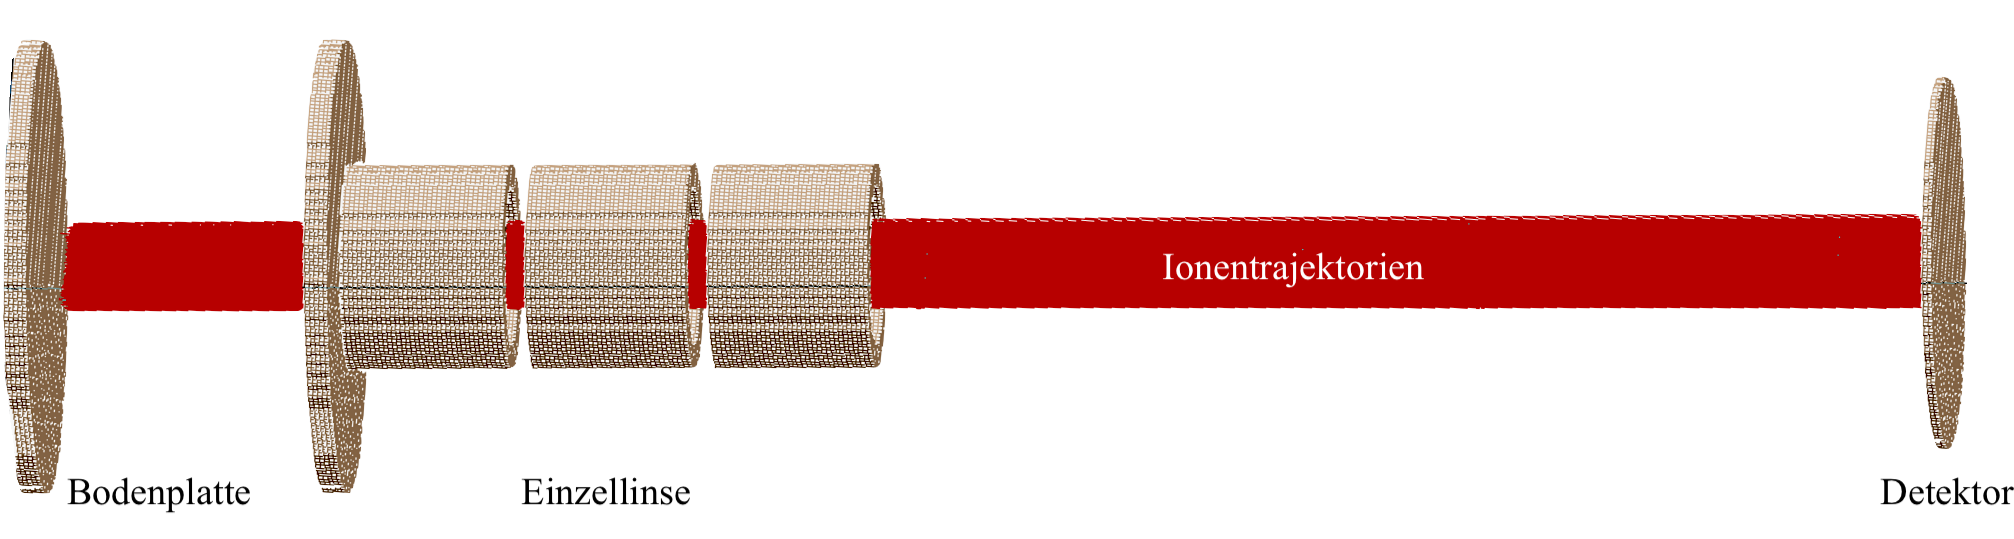
\includegraphics[width=1\textwidth]{Model.png}
    \caption[Modell des Massenspektrometers in \textsc{Simion}]{Modell des Massenspektrometers in \textsc{Simion}. Die Elektroden sind in Beige dargestellt, die Flugbahnen der Ionen in Rot. Dargestellt ist die Geometrie einer Flugstrecke von 410 mm.}
    \label{fig:model}
\end{figure}

Auf der Bodenplatte (in der Simulation links) wird ein positives Potential von mehreren Kilovolt angelegt, während die Deckenplatte und Einzellinse auf Masse (0 V) liegt. Genauso wie im Experiment wird die Linse vorerst nicht verwendet. Der Detektor (in der Simulation rechts) bekommt ein Potential von -2500 V, ähnlich dem in der Anlage. 

\subsection{Initialisierung der Ionen}
Die Interaktion der Elektronen mit dem Neutralgas wird in der Simulation nicht berücksichtigt. Stattdessen werden die Ionen im Pfad des Elektronenstrahls erschaffen, also in einem Streifen parallel zu den Platten. Um die räumliche Ausdehnung des Strahls zu berücksichtigen und, wie auch im Experiment zu beobachten, eine Verteilung der Flugstrecken der Ionen zu erhalten, wird das in der Auswertung des Strahlprofils bestimmte Profil des Elektronenstrahls genutzt. Die Ionen werden dann mit einer FWHM von $1.95$ mm um die Linie des Strahls gauß-verteilt. Da das Experiment von der Einzelstoßbedingung ausgeht, kann ein Ion nach dem Anderen simuliert werden und die Wechselwirkung zwischen Ionen vernachlässigt werden.

Die Art der Teilchen sowie ihre Häufigkeitsverteilung, können mit einem \textsc{.fly2}-File definiert werden. Auch die räumliche Verteilung des Strahls wurde hierüber implementiert. Die verwendete Datei ist im Anhang \ref{fly2} zu finden. Für die kinetische Energie der Teilchen wird 1/40 eV aufgrund thermischen Bewegung angenommen. Dieser Wert ergibt sich, wenn man eine Maxwell-Boltzmann-Verteilung für die kinetische 
Energie der Ionen annimmt und die Temperatur der Ionen auf 300 K (Raumtemperatur) setzt: 
\begin{equation}
    \label{eq:kin}
    \left< E_{\text{Kin}} \right> = \frac{3}{2} k_\mathrm{B} T_\mathrm{Raum} \approx \frac{1}{25} \text{ eV}.
\end{equation}

\subsection{Extraktion der Ionen}
Die Extraktion der Ionen erfolgt durch die Anlegung eines elektrischen Feldes zwischen den Platten, analog zum Experiment. Damit der Vergleich so präzise wie möglich ist, wird das Potential auf der Bodenplatte zeitabhängig verändert. Dabei wird die Spannung von 0 auf 5000 V mit einer linearen Rampe in 50 ns erhöht, nachdem die Extraktionsverzögerung abgewartet wurde. Die Zeitabhängigkeit wurde dem Signalverlauf (dargestellt in \ref{fig:Signal}) entnommen. Die Ionen werden dann in einem Zeitfenster von 4 $\mu$s extrahiert. Um das zeitabhängige Potential umzusetzen, wird ein \textsc{Workbench}-File genutzt, das die Spannung in Abhängigkeit der Zeit definiert. In \textsc{Simion} können Potentiale angepasst werden, ohne das gesamte Potential-Array neu berechnen zu müssen. Dies ist möglich, da die Potentiale durch eine Überlagerung von Spannungen auf bereits existierenden Elektroden definiert sind.

\section{Vergleich der Simulation mit dem Experiment}
Um dieselben Informationen aus der Simulation zu gewinnen, wie sie auch im Experiment vom Detektor aufgenommen werden, werden Flugzeit und Position jedes Teilchens zum Auftreffpunkt aufgezeichnet. Diese können dann mit denselben Methoden wie die experimentellen Daten ausgewertet werden. Im Folgenden werden verschiedene Simulationen durchgeführt, um die Ionenoptik zu untersuchen. Dafür sollen zunächst die Ergebnisse aus dem Experiment nachsimuliert werden, um die Genauigkeit der Simulation zu überprüfen. 


\begin{figure}
    \centering
    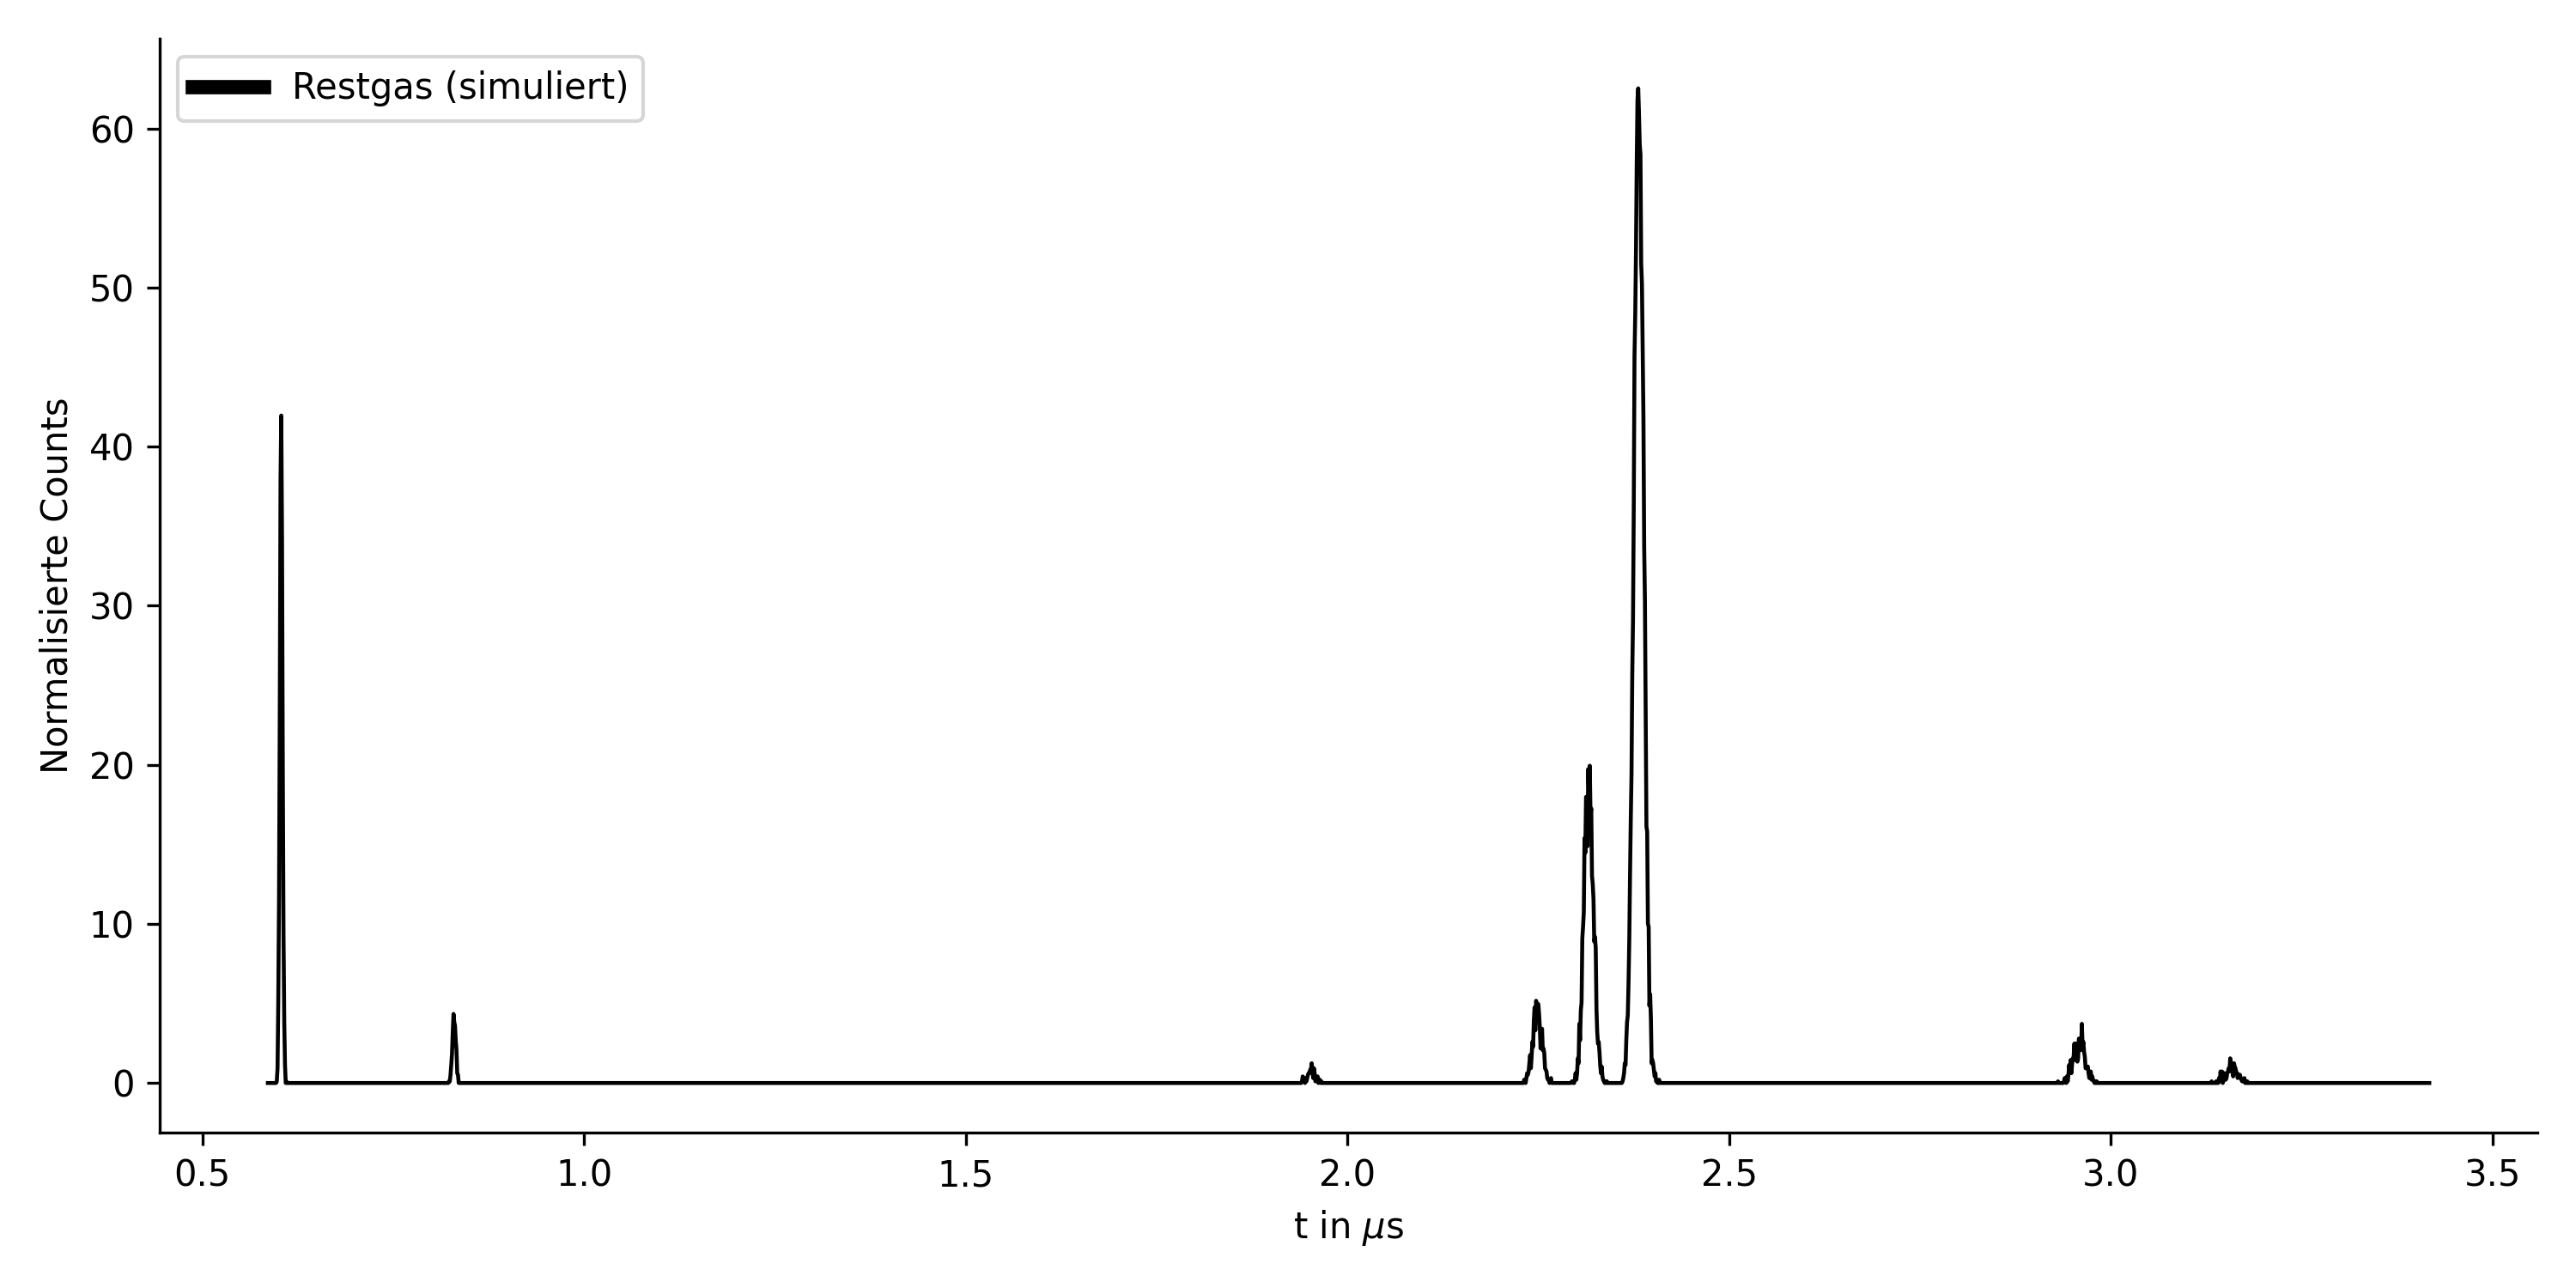
\includegraphics[width=1\textwidth]{Restgas_Sim.png}
    \caption[Simuliertes Restgasspektrum]{Ein simuliertes Restgasspektrum, die Ionenverteilung wurde anhand der Auswertung des Restgasspektrums gesetzt.}
    \label{fig:Restgas_Sim}
\end{figure}

Implementiert man eine Ionenverteilung ähnlich der in der Auswertung des Restgasspektrums bestimmten, kann man ein vergleichbares Flugzeitspektrum aus simulierten Daten generieren. Abbildung \ref{fig:Restgas_Sim} zeigt ein solches Ergebnis. Die Flugzeitverteilung der Ionen ist ähnlich der im Experiment beobachteten. Die zeitliche Abweichung der simulierten Peaks zu den echten Daten beträgt weniger als 100 ns und kommt wahrscheinlich durch die vereinfachte lineare Umsetzung der kapazitiven Beschleunigungsplatte zustande. In der Simulation wird bestätigt, dass die Ionen in einem Zeitfenster von 4 $\mu$s extrahiert werden. Die Peaks sind schärfer als im Experiment und es ist deutlich weniger Rauschen vorhanden. Das liegt daran, dass die Simulation keine Störeffekte berücksichtigt und der Detektor idealisiert ist. Dass das Ergebnis kein Linienspektrum ist, liegt daran, dass der Strahl als räumlich ausgedehnt simuliert wird.

\begin{figure}[H]
    \centering
    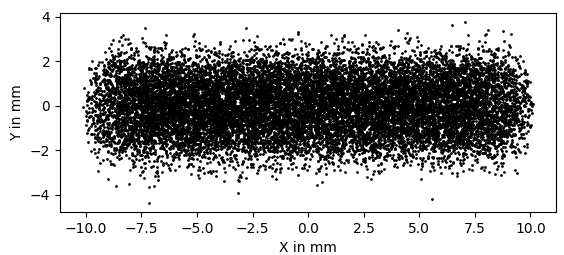
\includegraphics[width=.8\textwidth]{Sim_Positions_Scatter.png}
    \caption[Streudiagramm der simulierten Ionenposition auf dem Detektor]{Die Position der Ionen auf dem Detektor als Streudiagramm ohne Diskretisierung.}
    \label{fig:sim_pos_scatter}
\end{figure}

Nicht nur die Flugzeit, sondern auch die räumliche Verteilung der Ionen kann mit der Simulation überprüft werden. Dafür wird die Position der Ionen beim Auftreffen auf den Detektor aufgezeichnet. Abbildung \ref{fig:sim_pos_scatter} zeigt ein Streudiagramm der Orte. Da anders als in der Realität keine Auflösungsbegrenzung durch den Detektor existiert, ist die räumliche Auflösung der Punkte lediglich durch die Genauigkeit der Darstellung in \textsc{Simion} begrenzt.

Um vergleichbare Daten zu erhalten, wird der Ort diskretisiert. Die Detektorfläche wird in 280 x 280 Pixel unterteilt und in Abbildung \ref{fig:sim_pos_both}, wie auch in der Auswertung, dargestellt. Auffällig ist, dass die Ionen in der Simulation einen kürzeren Streifen einnehmen als im Experiment. Die Länge des Abbilds des simulierten Strahls ist mit etwa 24 mm kürzer als der 28 mm lange Streifen aus dem Experiment. Eine Überhöhung an den Rändern des Strahls ist in der Simulation nicht zu erkennen.

Die Aufweitung des Strahls ist mit der thermischen Bewegung der Ionen zu erklären. Um diesen Zusammenhang sichtbar zu machen, sind in Abbildung \ref{fig:sim_pos_both} die Auftrefforte der Ionen bei unterschiedlichen kinetischen Energien dargestellt. Erhöht man die kinetische Energie der Teilchen sieht man, dass das Abbild des Strahls deutlich breiter, nicht aber viel länger wird (Abb. \ref{fig:sim_pos_kinetic}). Die Länge von 28 mm wird nicht erreicht. Beim Vergleich mit den Dimensionen aus der Auswertung ist eindeutig, dass die Annahme von 1/25 eV deutlich näher an den experimentellen Daten liegt. 

\begin{figure}
    \centering
    \begin{subfigure}{.43\textwidth}
        \centering
        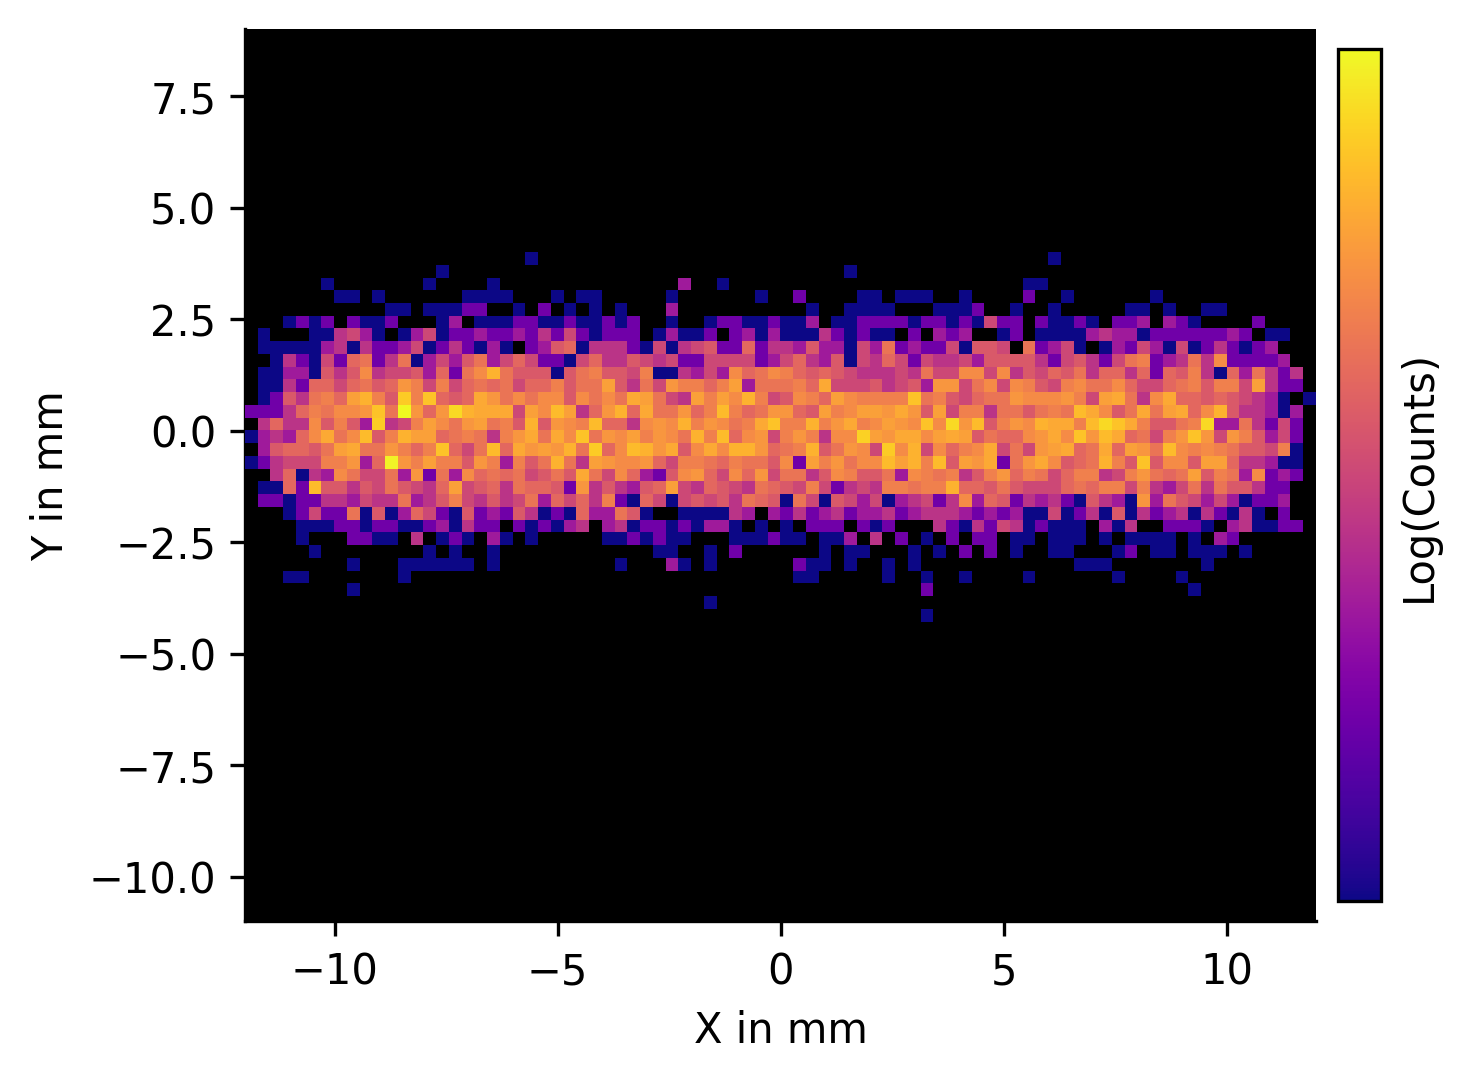
\includegraphics[width=1\textwidth]{Sim_Positions.png}
        \caption{Ionen bei 1/25 eV kinetischer Energie}
        \label{fig:sim_pos}
    \end{subfigure}%
    \hfill
    \begin{subfigure}{.45\textwidth}
        \centering
        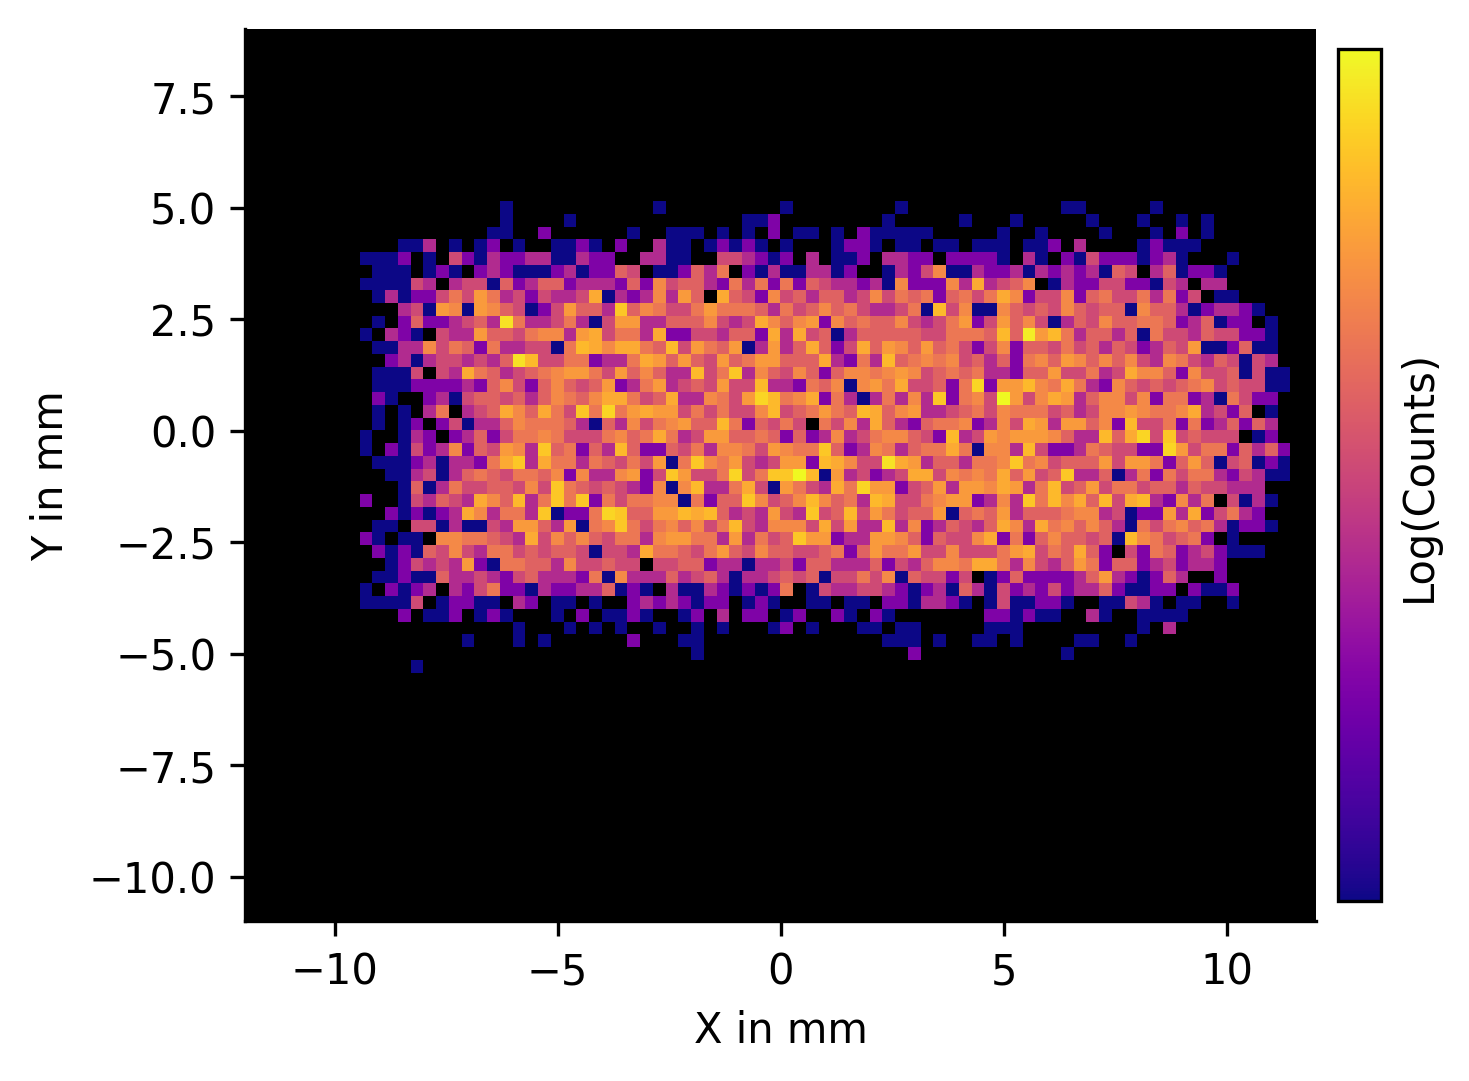
\includegraphics[width=1\linewidth]{Sim_Positions_Kinetic.png}
        \caption{Ionen bei 1/5 eV kinetischer Energie}
        \label{fig:sim_pos_kinetic}
    \end{subfigure}
    \caption[Simuliertes Abbild des Strahls auf dem Detektor bei verschiedenen Energien]{Logarithmisches Abbild des simulierten Strahls auf dem Detektor bei unterschiedlichen kinetischen Energien. Die Länge des tatsächlichen Strahls ist als Vergleich eingezeichnet. Die Bilder sind deutlich weniger gesättigt, da nicht annähernd so viele Ionen simuliert wurden, wie im Experiment über einen längeren Zeitraum gesammelt wurden. Einen Hintergrund wie im Experiment gibt es in der Simulation nicht.}
    \label{fig:sim_pos_both}
\end{figure}

Anhand dieser Vergleiche kann bereits festgestellt werden, dass die Simulation der Ionenoptik in \textsc{Simion} eine gute Übereinstimmung mit den experimentellen Daten zeigt, auch wenn nicht alle Phänomene abgebildet werden können. Die Simulation kann also genutzt werden, um die Ionenoptik des Massenspektrometers zu untersuchen und Optimierungsansätze zu finden.

\section{Untersuchung der Ionenoptik}
Die folgende Untersuchung der Ionenoptik soll verschiedene Optimierungsansätze für das Massenspektrometer liefern. Dafür wurden geometrische Parameter variiert und die Auswirkungen auf die Flugzeit und die Position der Ionen auf dem Detektor untersucht. Besonders interessant ist der Einfluss der Flugstrecke auf die Flugzeitverteilung. Außerdem soll die Energie-Flugzeit-Korrelation untersucht werden und die Energieauflösung des Massenspektrometers zu bestimmen.

\begin{figure}
    \centering
    \begin{subfigure}{.9\textwidth}
        \centering
        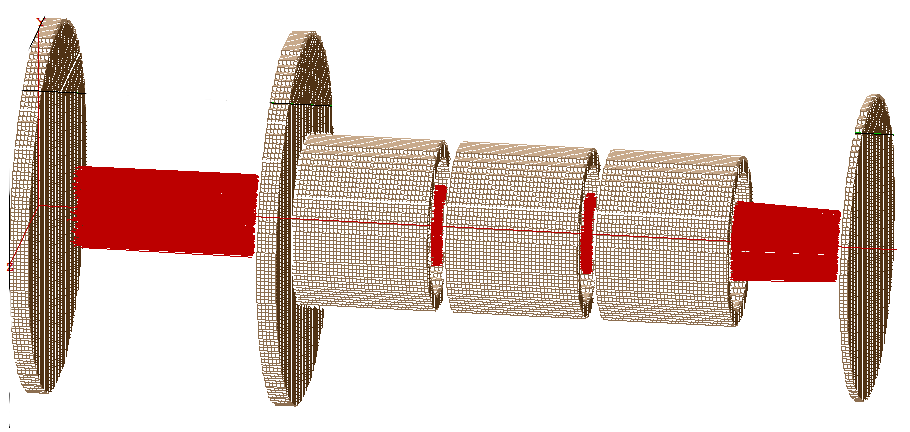
\includegraphics[width=.8\textwidth]{210_3D.png}
        \caption{Die Trajektorien der Ionen in 3D. Ein konvergenter Strahl ist in nähe des Detektors (rechts) zu erkennen.}
        \label{fig:210}
    \end{subfigure}%
    \vfill
    \begin{subfigure}{.9\textwidth}
        \centering
        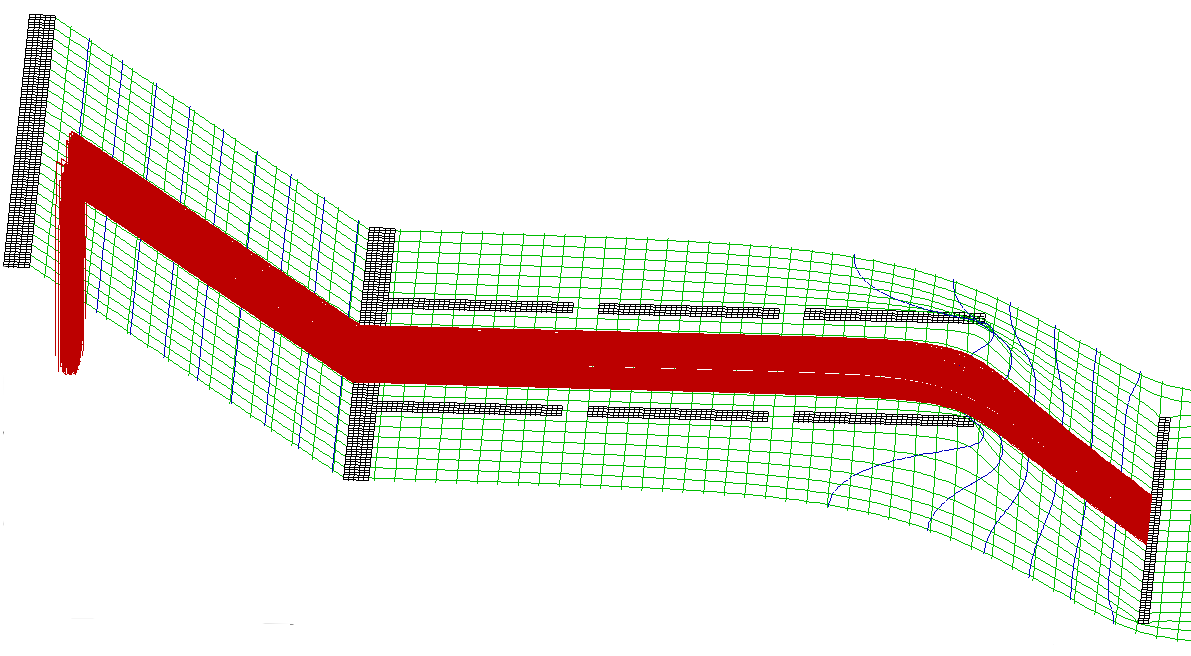
\includegraphics[width=.8\textwidth]{PE.png}
        \caption{Darstellung der potentiellen Energie in 3D. Das Potential wird vom grünen Gitter dargestellt. Äquipotentiallinien sind in Blau eingezeichnet.}
        \label{fig:PE}
    \end{subfigure}
    \caption[Simulation mit verkürzter Flugstrecke]{Simulation mit verkürzter Flugstrecke. Trajektorien der Ionen sind in Rot dargestellt.}
    \label{fig:210_PE}
\end{figure}

\subsection{Einfluss der Flugstrecke}
Alle bisher gezeigten Spektren wurden bei einer gesamten Flugstrecke von etwa 41 cm aufgenommen. Der Abstand des Beschleunigungskondensators ist bei 6 cm festgelegt. Diese Strecke ist fast vollständig in der Flugstrecke inkludiert, da der Elektronenstrahl den Kondensator in der Nähe (6 mm Entfernung) der Bodenplatte durchquert. Um den Einfluss der Flugstrecke zu untersuchen, wurden Simulationen mit 21 cm, etwa der Hälfte der Strecke, durchgeführt. Dafür ist der Detektor um 20 cm verschoben worden. Abbildung \ref{fig:210_PE} zeigt die Geometrie sowie das Potential in der Simulation mit der verkürzten Strecke. Es ist zu erkennen, dass der Strahl deutlich auf den Detektor fokussiert wird. Schaut man sich \ref{fig:PE} an, so sieht man, dass die Einzellinse, die komplett auf Masse liegt, aufgrund der hohen Potentialdifferenz zum Detektor bei -2500 V eine starke Fokussierung der Ionen bewirkt. Dieser Effekt ist sehr viel stärker als bei der größeren Entfernung. 

Ein Vergleich der Masse-zu-Ladungsspektren ist in Abbildung \ref{fig:410_210} zu sehen. Es ist ein deutlicher Unterschied in der Schärfe der Peaks sichtbar. Besonders bei der Auswertung der höhergeladenen Argonionen sind die Daten der kleineren Geometrie höherwertig. Der TPHC müsste aufgrund der verkürzten Flugzeit auf ein Maximum von 3 $\mu$s eingestellt werden. Nicht beachtet wurde hierbei, dass der Fehler bei der Bestimmung der Flugzeit mit dem realen TPHC einen prozentual höheren Einfluss hätte. Die Simulation zeigt, dass eine kürzere Flugstrecke zu einer besseren Auflösung des Massenspektrometers führt. Ein Positionsplot bestätigt den konvergenten Strahl, der auf den Detektor fokussiert wird. Das Abbild des Strahls ist nur noch etwa 20 mm lang. Er ist im Anhang \ref{fig:pos_210} zu finden.

\begin{figure}
    \centering
    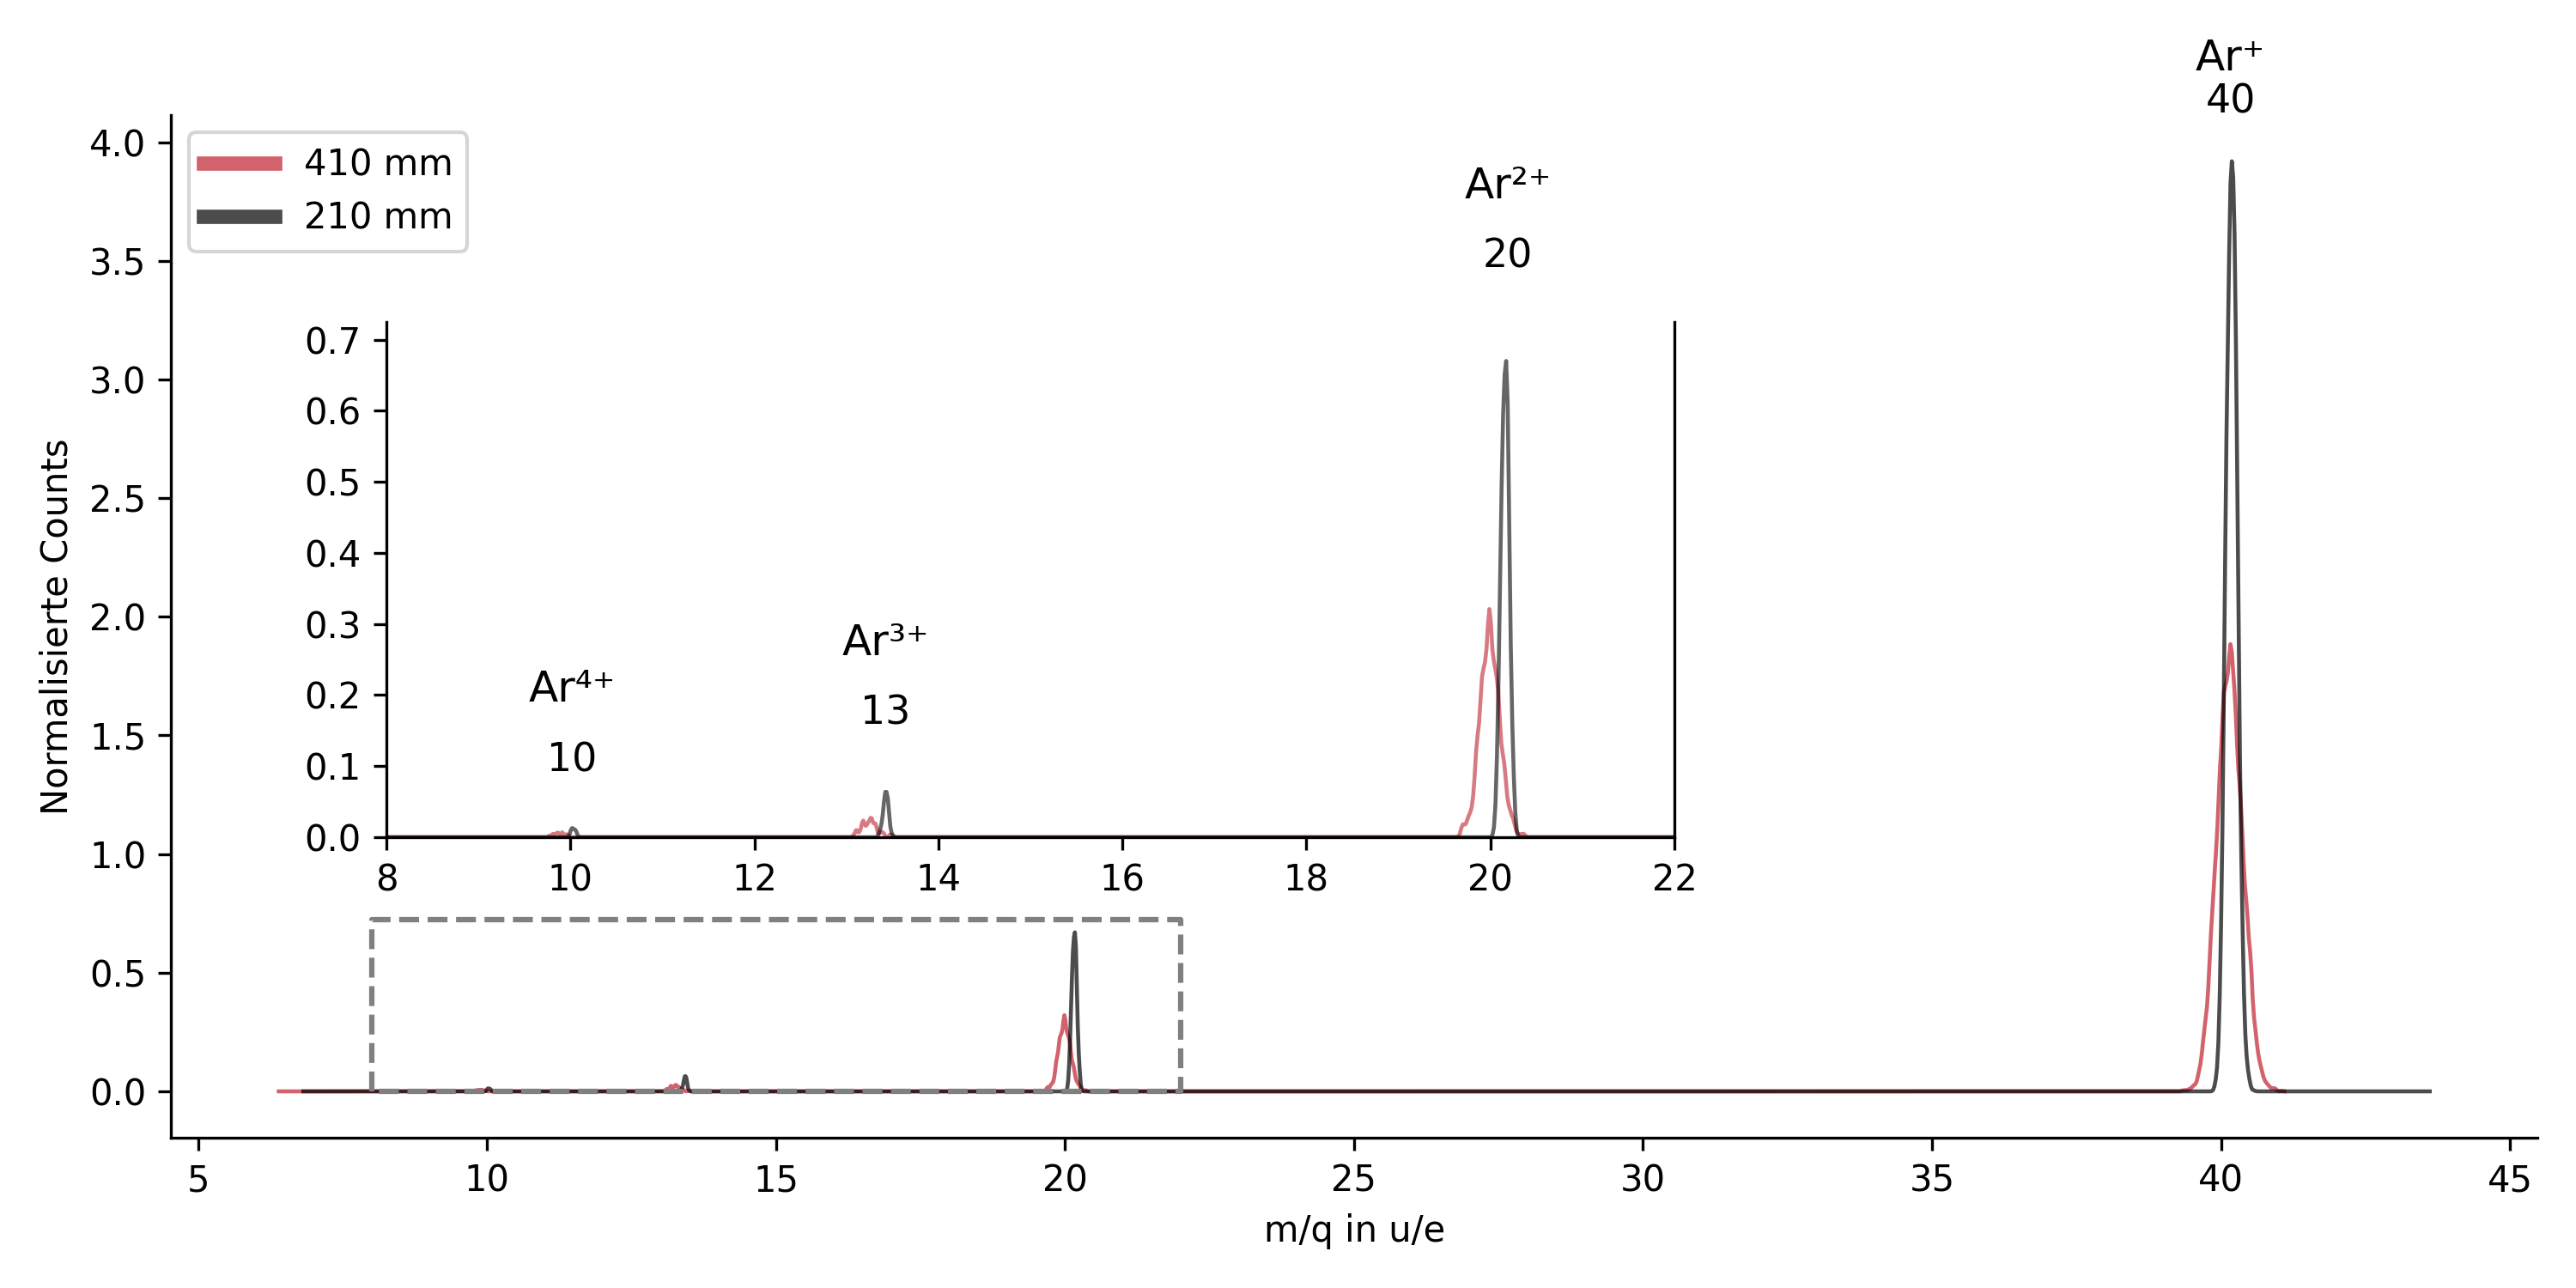
\includegraphics[width=1\textwidth]{410_210_Ar1000eV.png}
    \caption[Vergleich der Masse-zu-Ladungsspektren bei unterschiedlichen Flugstrecken]{Vergleich der Masse-zu-Ladungsspektren bei unterschiedlichen Flugstrecken. In Schwarz wurde die kürzere Distanz dargestellt. Die Flugzeitspektren wurden mit unterschiedlichen Transformationsfunktionen umgerechnet, da die kürzere Distanz die Flugzeit deutlich verkürzt. Die Ionenverteilung entspricht der in der Auswertung bestimmten für Argon bei 1000 eV.}
    \label{fig:410_210}
\end{figure}
\subsection{Untersuchung der Anomalien}
Der im Experiment gefundene Zusammenhang zwischen der eingestellten Elektronenenergie und der Flugzeit der Ionen kann nicht direkt in der Simulation überprüft werden, da die Elektronen selbst nicht simuliert werden. Trifft man die Annahme, dass die überschüssige kinetische Energie der Elektronen auf die Ionen übertragen wird, würde man erwarten in der Simulation einen ähnlichen Zusammenhang zu sehen. Dafür wurden verschiedene Simulationen mit unterschiedlichen kinetischen Energien der Ionen durchgeführt. Nach ausgiebiger Prüfung konnte kein Zusammenhang zwischen der kinetischen Energie der Ionen und der Flugzeit gefunden werden. Die Flugzeit der Ionen ist unabhängig von ihrer kinetischen Energie, mit einer kürzeren Extraktionsverzögerung kann lediglich die Peakbreite verändert werden. Daraus lässt sich schließen, dass die Verzögerung auf einen anderen Effekt vor der Ionisierung zurückzuführen ist. 

Durch die Untersuchung der räumlichen Verteilung der Produktionen wird deutlich, dass ein in der Simulation nicht berücksichtigter Effekt Ursache für die Anomalien im Abbild sein muss. Das bestärkt die Vermutung, dass es zur Wechselwirkung zwischen den Ionen kommt. Wie bereits in \ref{sec:Anomalien} erwähnt, ist es auch bei kontrollierter Produktrate nicht unmöglich, dass innerhalb eines Elektronenpulses mehrere Ionisationsprozesse stattfinden. Die Coloumbabstoßung zwischen den Ionen könnte dann zu einer Aufweitung des Strahls und zu einer Überhöhung am Rand führen. Um diesen Effekt zu untersuchen, müsste eine Simulation mit mehreren Ionen pro Elektronenpuls durchgeführt werden. Wie in \ref{chap:Simulation} erwähnt, ist das in \textsc{Simion} möglich, aber aufgrund der erhöhten Rechenzeit nur für wenige Ionen sinnvoll. Simulationen mit zwei bis vier Ionen mit verschiedenen Ladungen pro Elektronenpuls zeigen jedoch, dass die Abstoßung der Ionen gegenüber der Beschleunigung auf den Detektor nicht stark genug ist, um die beobachteten Effekte zu erklären. Für einen sichtbaren Effekt müssten die Ladungen der Ionen deutlich höher sein und die Flugzeit um ein Vielfaches länger. Auch dieser Effekt kann also nicht die Ursache für die beobachteten Anomalien sein.

\label{sec:delay}
\subsection{Auflösungsvermögen}
Das Auflösungsvermögen eines Massenspektrometer beschreibt, wie gut es in der Lage ist, zwei Ionen mit ähnlicher Masse als getrennte Peaks aufzulösen. Ein hohes Auflösungsvermögen ist besonders wichtig, wenn man Isobare, also Elemente mit nahezu identischen Massen, unterscheiden möchte. Für die Untersuchung der meisten Gase in dieser Anlage ist kein besonders hohes Auflösungsvermögen gefordert. Dennoch ist es sinnvoll zu überprüfen, wie hoch das Auflösungsvermögen ist und dieses zu quantifizieren. Mithilfe der Simulation kann das theoretisch erreichbare Auflösungsvermögen bestimmt werden. 

Das Auflösungsvermögen ist definiert als 
\begin{equation}
    R = \frac{m}{\Delta m},
    \label{eq:res}
\end{equation}
wobei $m$ die mittlere Masse und $\Delta m$ die FWHM eines Peaks im Massenspektrum ist. Um es zu bestimmen, können in der Simulation Testmassen von 1 bis 60 $u$ in 1 $u$ und 0.5 $u$ Schritten simuliert werden. Diese werden jeweils einfach geladen und ihre Flugzeit aufgezeichnet. Ein Massenspektrum, dargestellt in Abbildung \ref{fig:res}, ergibt sich nach Transformation der Flugzeitdaten.

\begin{figure}
    \centering
    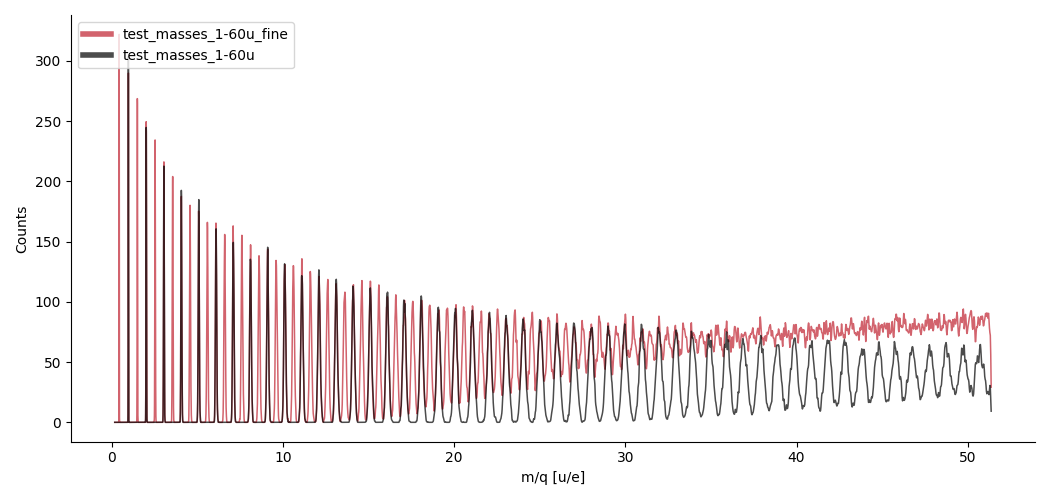
\includegraphics[width=1\textwidth]{Resolution.png}
    \caption[Simuliertes Massenspektrum (1–60 u, 410 mm) zur Auflösungsbestimmung]{Simuliertes Massenspektrum der Massen 1 bis 60 $u$ (einfach geladen) zur Bestimmung des Auflösungsvermögens bei einer Detektordistanz von 41 cm. Alle Spezies sind mit der gleichen Häufigkeit vertreten. In Schwarz sind die Peaks für ganzzahlige Massen, in Rot auch die für halbzahlige dargestellt.}
    \label{fig:res}
\end{figure}

Ein Zusammenhang zwischen der Schärfe der Peaks und der Masse ist sofort erkennbar. Mit steigender Masse nimmt die FWHM zu. Die Korrelation kommt daher, dass die prozentuale Massen- und damit auch die Flugzeitdifferenz ähnlicher Ionen mit steigender Masse abnimmt. So entspricht beispielsweise das Verhältnis der Flugzeiten von 1 zu 2 $u$ 38 \% und das von 29 zu 30 $u$ nur 1.8 \% bei einfacher Ladung. Bei höheren Flugzeiten verschmelzen die Peaks teilweise, sodass eine Identifikation einzelner Häufigkeiten nicht mehr möglich ist. Die Breite der Peaks hängt dabei vor allem von der Breite des Elektronenstrahls ab, da dieser den Entstehungsort der Ionen bestimmt. Auch die Distanz des Detektors hat jedoch einen maßgeblichen Einfluss auf das Auflösungsvermögen. Eine kürzere Flugstrecke und damit Flugzeit führt dazu, dass kleine Geschwindigkeitsunterschiede nicht in signifikante Flugzeitunterschiede umgewandelt werden.

\begin{figure}
    \centering
    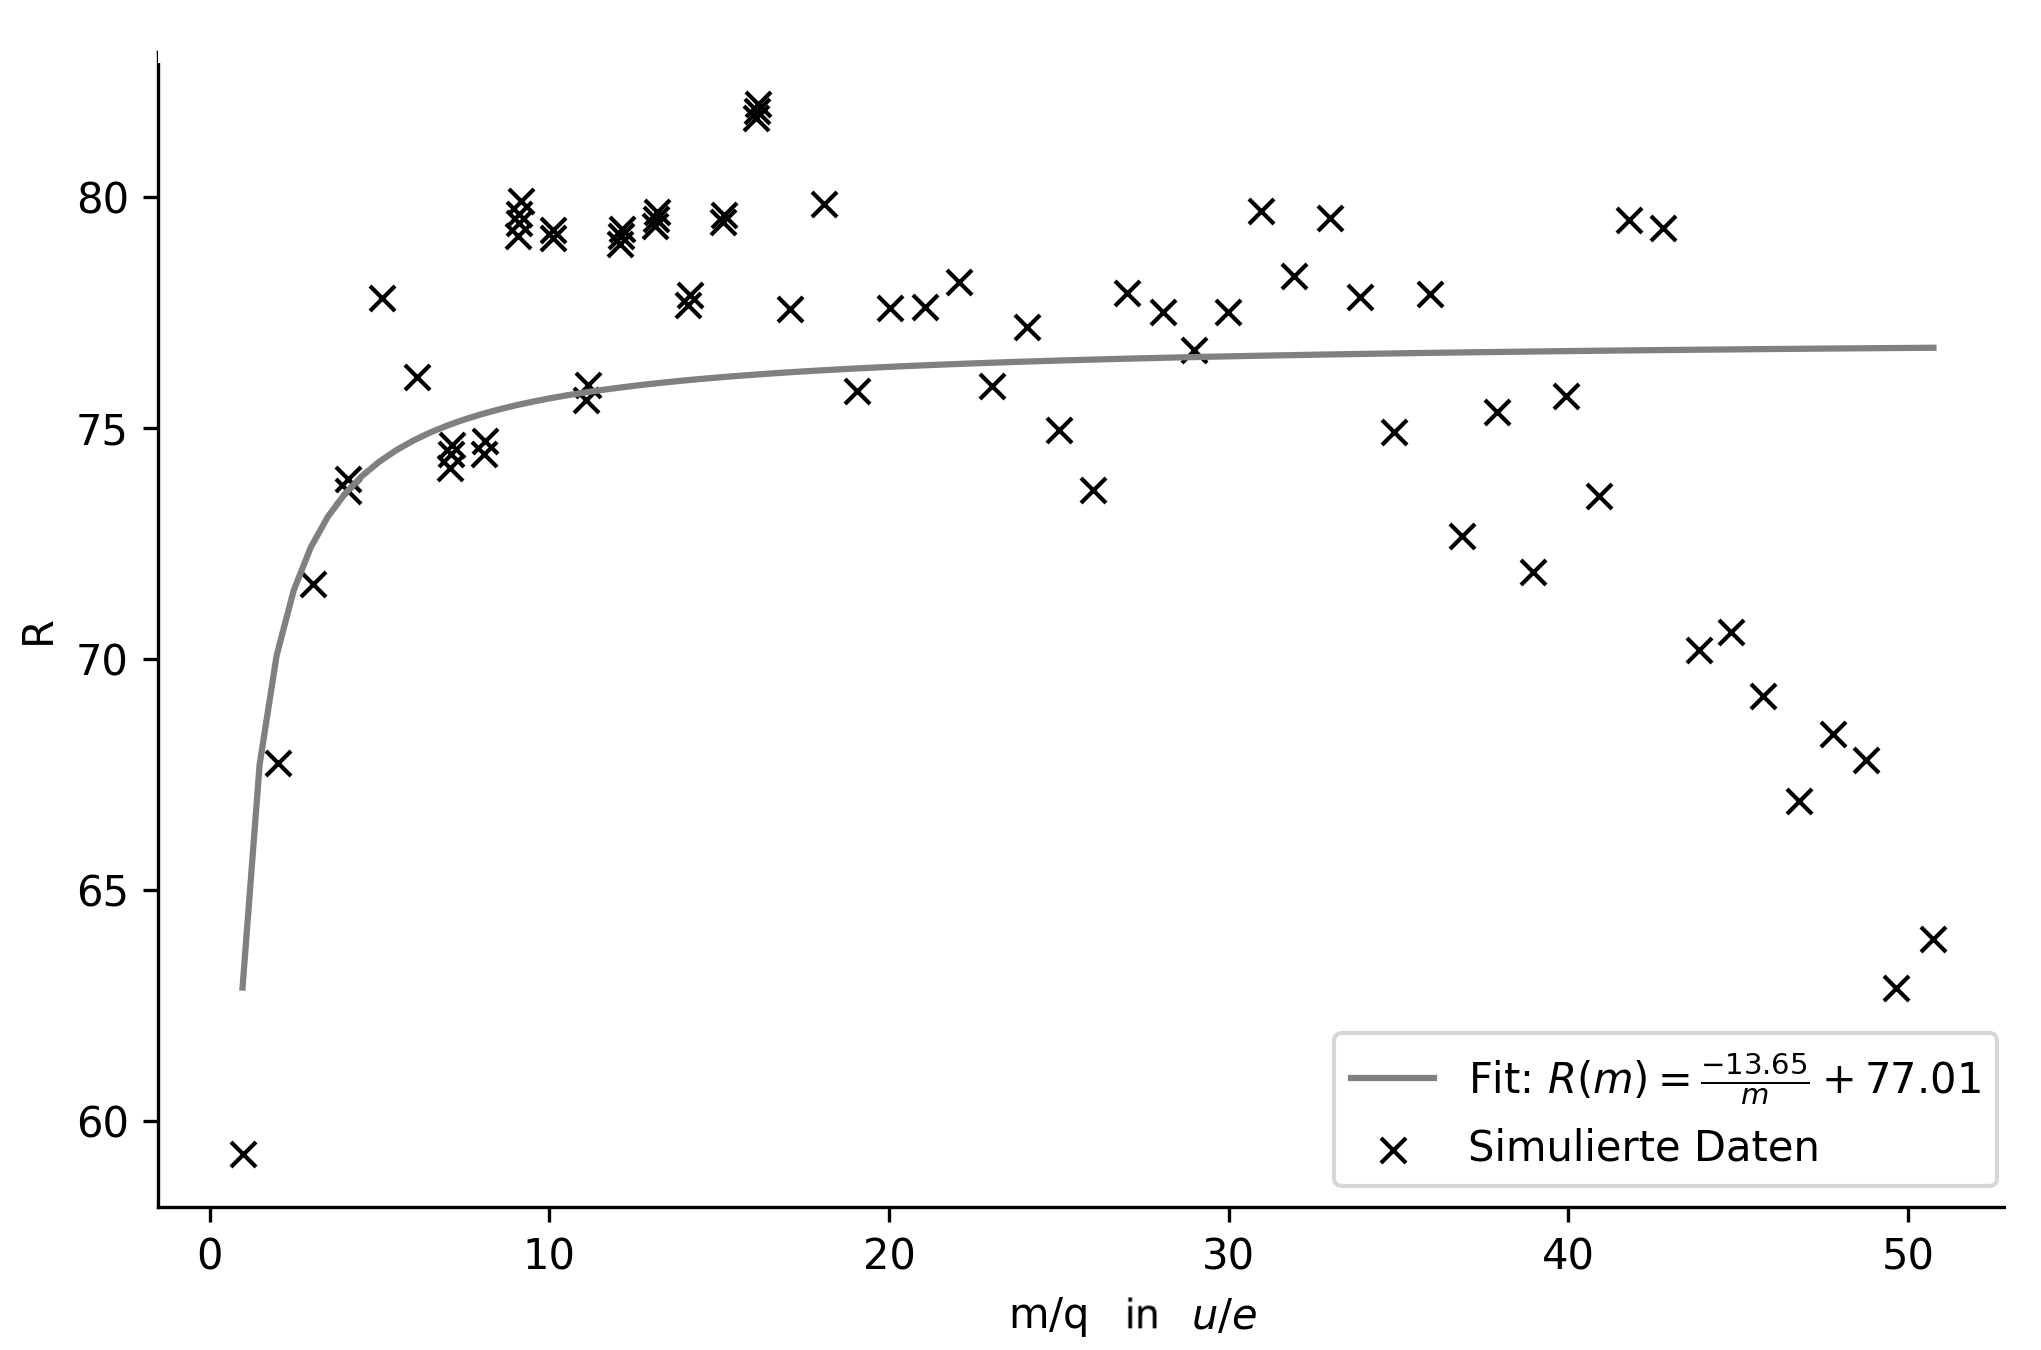
\includegraphics[width=.9\textwidth]{ResolutionFit.png}
    \caption[Auswertung des Auflösungsvermögens abhängig von der Masse (410 mm)]{Auswertung des Auflösungsvermögens abhängig von der Masse. Die Datenpunkte sind die Verhältnisse der mittleren Massen und der FWHM der Peaks eines simulierten Spektrums.}
    \label{fig:res_fit}
\end{figure}

Eine Auswertung des Massenspektrums ist möglich, indem alle Peaks mit einer Gaußfunktion gefittet werden und ihr FWHM errechnet wird. Das Auflösungsvermögen kann dann abhängig von der Masse mit Formel \ref{eq:res} ausgerechnet und dargestellt werden. Abbildung \ref{fig:res_fit} zeigt das Ergebnis abhängig von der Masse. Anders als erwartet steigt das Auflösungsvermögen zunächst mit steigender Masse, wobei es einem reziproken Verlauf folgt (Fit). Ab einer Masse von etwa 10 $u$ ist es weitestgehend konstant und liegt bei etwa 75. Das bedeutet, dass sich die Masse zweier Peaks um mindestens 1/75 der Masse einer der Peaks unterscheiden muss, damit sie als getrennte Peaks identifiziert werden können. Ab einer Masse von etwa 35 $u$ fällt das Auflösungsvermögen wieder ab. Die Peaks werden hier schneller breiter, als die Massenunterschiede zunehmen. Das Auflösungsvermögen ist also nicht konstant, sondern hängt von der Masse der Ionen ab, wobei sein Optimum zwischen 5 und 35 $u$ liegt.

\begin{figure}
    \centering
    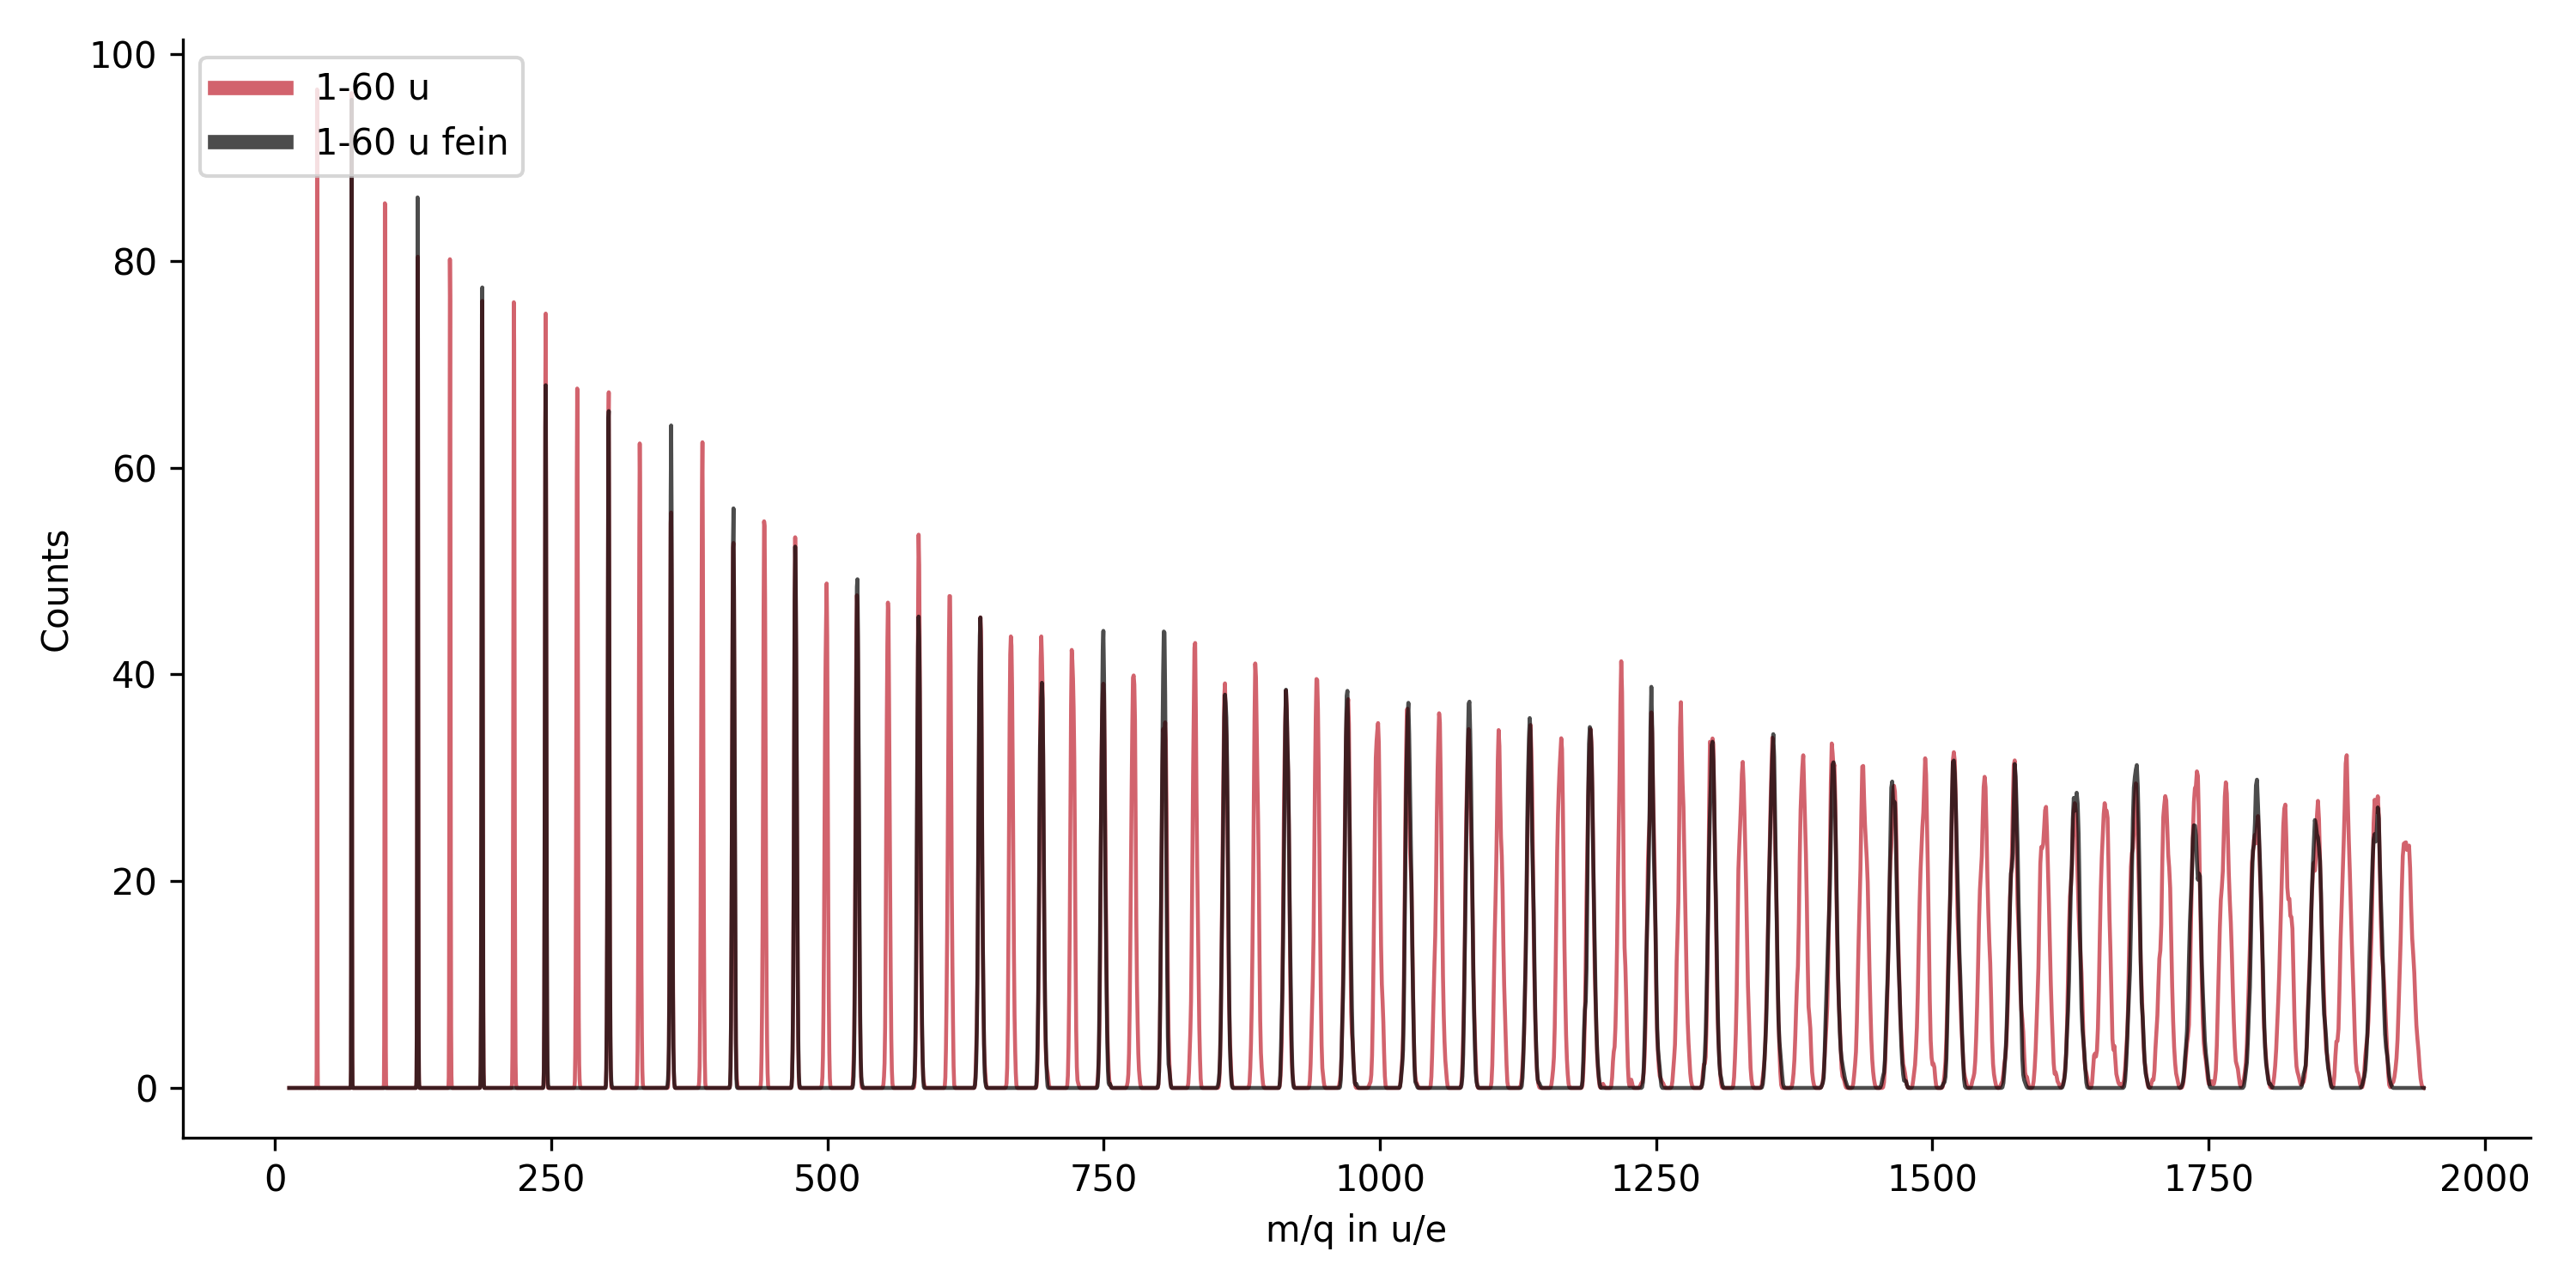
\includegraphics[width=1\textwidth]{Resolution210.png}
    \caption[Simuliertes Massenspektrum (1–60 u, 210 mm) zur Auflösungsbestimmung]{Simuliertes Massenspektrum wie in Abbildung \ref{fig:res} zur Bestimmung des Auflösungsvermögens bei einer Detektordistanz von 21 cm. Die Peaks sind deutlich schärfer.}
    \label{fig:res21}
\end{figure}

\begin{figure}
    \centering
    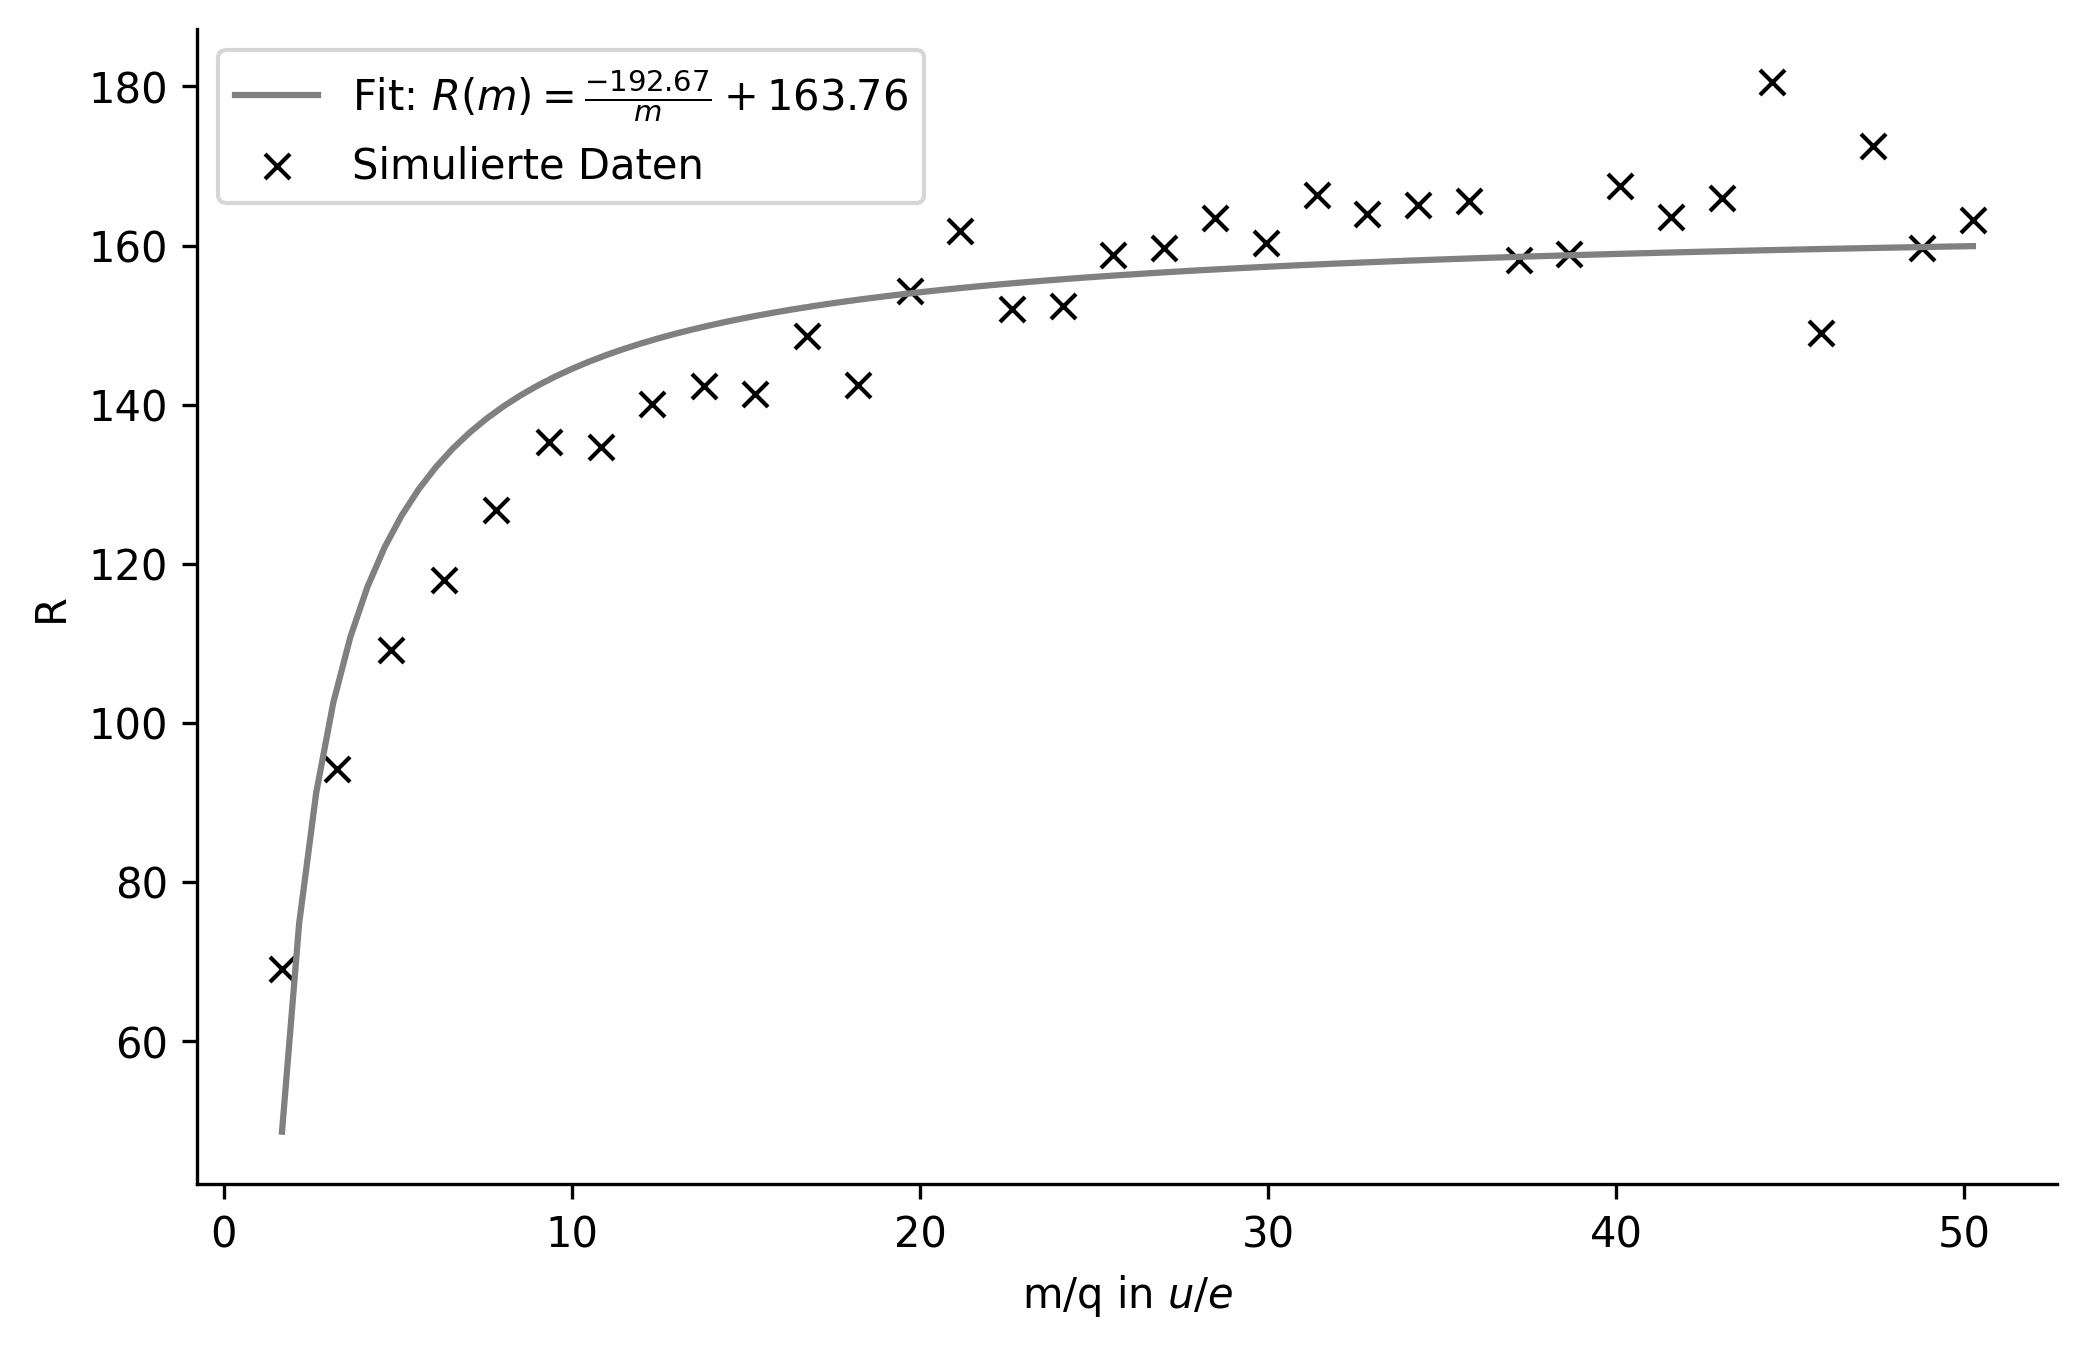
\includegraphics[width=.9\textwidth]{ResolutionFit210.png}
    \caption[Auswertung des Auflösungsvermögens abhängig von der Masse (210 mm)]{Auswertung des Auflösungsvermögens abhängig von der Masse bei einer Detektordistanz von 210 mm.}
    \label{fig:res_fit210}
\end{figure}

Abbildung \ref{fig:res21} zeigt das gleiche simulierte Massenspektrum, jedoch bei einer Detektordis-tanz von 21 cm. Die Peaks sind viel schärfer, sodass auch bei einer Masse von 50 $u$ noch eine Auflösung von über 150 erreicht wird. Das Auflösungsvermögen ist in Abhängigkeit von der Masse in Abbildung \ref{fig:res_fit210} dargestellt. Der Verlauf ist ähnlich, jedoch ist das Auflösungsvermögen etwa doppelt so hoch und steigt noch bis über 60 $u$ an. Die Veränderung der Flugstrecke hat also einen großen Einfluss auf das Auflösungsvermögen der Anlage.

Vergleicht man die theoretisch mögliche Auflösung mit Werten aus dem Experiment, fällt auf, dass diese wie erwartet schlechter ist. Insgesamt sind die Peaks im Experiment weniger scharf, was auf die Idealisierung der Simulation und die Breite des Strahls zurückzuführen ist. Es ist nicht möglich ein Spektrum wie in Abbildung \ref{fig:res} aufzunehmen und direkt zu vergleichen. Der qualitative Verlauf des Auflösungsvermögens bei Auswertung eines Restgasspektrums ist jedoch ähnlich und etwa bei der Hälfte des Wertes.


\section{Diskussion und Ausblick}
Obwohl die Anlage mit einer Fehlfunktion der Elektronenkanone nur eingeschränkt genaue Messungen zulässt, können aus den gemessenen Daten einige Informationen in der Auswertung erarbeitet werden. Die Aufnahme von Argonspektren bei verschiedenen Elektronenenergien hat gezeigt, dass der neue Detektor sowohl zeitlich als auch räumlich sinnvolle Daten aufnehmen kann. Durch einen Vergleich mit Daten von Straub et al. \cite{Straub} und die Aufnahme eines Restgasspektrums kann verifiziert werden, dass die Anlage korrekt arbeitet und diese ausreichend gut qualitativ reproduzieren kann. 

Für die Auswertung wurden außerdem einige Skripte entwickelt, die die Transformation und Analyse von Flugzeitspektren vereinfachen. Dabei kann bestätigt werden, dass der Zusammenhang zwischen der Flugzeit und dem Masse-zu-Ladungsverhältnis der erwarteten Form entspricht.

Durch eine Untersuchung verschiedener Extraktionsverzögerungen kann eine deutliche Verbesserung in der Auflösung des Massenspektrometers mit einer Verzögerung von 600 ns erreicht werden. Dadurch kann nachvollzogen werden, dass die DETOF-Technik eine vorteilhafte Methode ist, um die Auflösung des Massenspektrometers zu verbessern und das diese mit korrekt dimensionierten Verzögerungszeiten auch bei \textsc{Zero-B} sinnvoll anwendbar ist.

Außerdem wurde ein bisher unbekannter Zusammenhang zwischen der Elektronenenergie und der Flugzeit der Ionen gefunden und seine Form beschrieben. Anhand der Positionsdaten des größeren Detektors ist es möglich ein gesamtes Abbild des Elektronenstrahls aufzunehmen und auszuwerten. Die Analyse der Positionsdaten liefert Informationen über das Elektronenstrahlprofil sowie die Trajektorien der Ionen. Dabei wurde bestätigt, dass die Ionen direkt mit dem Strahl korrelieren und anhand der Rate der Ionen die Einzelstoßbedingung kontrolliert. Trotzdem wurden bisher unzureichend untersuchte Effekte gefunden, wie die Überhöhung des Abbilds des Strahls an den Rändern und dessen Verbreiterung. Einige Gründe können mithilfe einer Simulation ausgeschlossen werden und Vermutungen über die Ursache angestellt werden, die weiteren Untersuchungen unterliegen sollten.

Die Simulation der Ionenoptik des Massenspektrometers in \textsc{Simion} hat gezeigt, dass das Programm eine gute Möglichkeit bietet, die Flugzeit und Trajektorien der Ionen zu untersuchen. Die Funktionsweise des Massenspektrometers kann nachgebildet werden und ist ausreichend verstanden, um die experimentellen Daten gut mit den simulierten vergleichen zu können. Ergebnisse aus dem Experiment können in großen Teilen reproduziert werden, was sowohl die \textsc{Zero-B} Anlage als auch die Simulation bestätigt und ihre Aussagekraft verbessert. Anhand der tatsächlichen Geometrie des Massenspektrometers können verschiedene Optimierungsansätze untersucht werden. Besonders erfolgreich wird gezeigt, dass durch die Verkürzung der Flugstrecke eine deutliche Verbesserung der Auflösung der \textsc{Zero-B} Anlage erreicht werden kann. 

Die in der Auswertung gefundenen Anomalien wurden mit der Simulation überprüft. Während eine geringfügige Aufweitung des Strahls durch die thermische Bewegung der Ionen bestätigt werden konnte, kann die Aufweitung des Strahls, die Überhöhung an den Rändern und die Energie-Flugzeit-Korrelation nicht in dem Maße nachvollzogen werden. Obwohl diese Effekte die Ergebnisse der Anlage nicht maßgeblich zu beeinflussen scheinen, sind sie dennoch interessant und sollten weiter untersucht werden. Möglich wäre es beispielsweise eine Testreihe bei deutlich kleineren Raten durchzuführen und zu überprüfen, ob das einen Einfluss auf die Überhöhungs- und Aufweitungseffekte haben könnte. Außerdem sollte nach Erneuerung der Elektronenkanone überprüft werden, ob die Energie-Flugzeit-Korrelation weiterhin besteht und ob sie mit dem Pulsieren der Gitterspannung zusammenhängen könnte.

Abschließen kann gesagt werden, dass die Weiterentwicklung der \textsc{Zero-B} Anlage im Rahmen dieser Arbeit erfolgreich umgesetzt wurde. Die Beschreibung zum Prinzip und Aufbau sowie die qualitativen Ergebnisse können als Grundlage genutzt werden, um mit der Anlage weitere Gase auf ihre Ionisationseigenschaften hin zu untersuchen. Die ionenoptische Simulation, die etabliert wurde, bietet zudem eine hilfreiche Beschreibung für die Validierung und Optimierung der Anlage. Mit ihr wurde im Rahmen dieser Bachelorarbeit quantifiziert, welche Verbesserungen die Verkürzung der Detektordistanz bringen können. Anhand dieses Ergebnisses wird die Anlage weiter optimiert werden. 
